\documentclass{article}
\usepackage[spanish]{babel}
\usepackage{graphicx} % Required for inserting images
\usepackage{float}

\title{Splatoon}
\author{Rafael Landeros Rodríguez}
\date{\today}

\begin{document}

\maketitle

\section{¿Qué es Splatoon?}

Básicamente Splatoon es el Shooter de Nintendo, donde controlas a un calamar o a un pulpo que dispara tinta y puedes nadar por el piso o la pared donde hayas pintado, y esta funny.\\

Esta saga contiene 4 juegos los cuales son:

\begin{enumerate}
    \item Splatoon
    \item Splatoon 2
    \item Splatoon 3
    \item Splatoon Raiders
\end{enumerate}

 \section{El lore antes de los juegos.}

La historia de splatoon empieza con la era contemporánea cuando los humanos vivían felices y contentos en la tierra, hasta que debido a la gran contaminación el cambio climático atacó aumentando la temperatura, haciendo que se derritan los polos por completo, esto causó que subiera el nivel del mar demasiado dejando que hubiera menos tierra en la cual habitar. \\

Lo anterior sumado a la sobrepoblación que había, provocó que se generadan innumerables guerras que terminaron con la raza humana, a excepción de un grupo de científicos que habían analizado la situación y se mudaron a una \textbf{cúpula} gigantesca bajo del mar, ahí sobrevivieron gracias a unos \textit{cristales que podían guardar memorias y ADN}, estos ayudaban a los sobrevivientes a recordar cómo era el mundo exterior antes de las guerras.\\

Y los humanos lograron sobrevivir un par de años en la cúpula hasta que nacieron las nuevas generaciones y estos no solo querían salir al mundo exterior si no de plano se querían ir a vivir al espacio, entonces construyeron un cohete y al intentar despejar destruyeron la cúpula (\textit{osea a quien se le ocurre despegar un cohete debajo del mar}) y ahora si se extinguieron todos los humanos.\\

Bueno aquí lo importante es que cuando se destruyó la cúpula fue que los cristales que guardaban recuerdos y ADN ahora quedaron en contacto con el agua, transmitiendo los recuerdos y el ADN a las criaturas marinas que se encontraban cerca, esto provocó que de poco a poco los seres marinos fueran evolucionando hacia una forma más humanoide y ganando una gran inteligencia, los que mejor se adaptaron con estas características fueron los \textbf{pulpos y calamares}, quienes fueron las especies dominantes.\\

\begin{figure}[H]
    \centering
    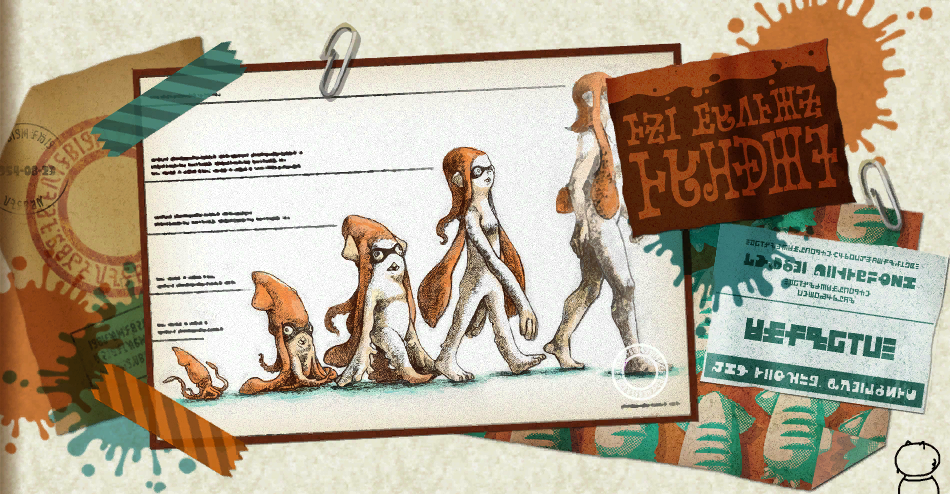
\includegraphics[width=1\linewidth]{image.png}
    \caption{Registro de como evolucionaron los calamares}
    \label{fig:placeholder}
\end{figure}

Ya en un punto evolucionaron tanto que ya ni siquiera podían vivir en el agua y empezaron a vivir en la superficie, así era la vida tranquila en la superficie donde ahora los seres marinos vivían en paz y armonía, sobre todo los \textbf{pulpos y calamares} mantenían una buena relación de amistad, pero hay que recordar que quedaba poca tierra y se incrementa muy rápido la población, esto primero lo notaron los pulpos y le declararon la guerra a los calamares para tener su territorio.\\

En esta guerra los pulpos siempre superaron a los calamares, y casi al final de la guerra ya casi estaban extintos los calamares, pero como ambos bandos ya había sufrido muchas bajas y había durado mucho la guerra decidieron hacer un \textit{gol gana}, literalmente una última batalla para decidir al vencedor, la cual lo ganaron los calamares, esto provocó que los pulpos fueran exiliados de la superficie obligándolos a vivir bajo tierra. 

\section{El lore ya en los juegos}

El primer Splatoon sucede años después de la guerra, los calamares dominaban la superficie mientras que los pulpos vivían en la pobreza bajo la tierra, ya que no tenían acceso libre a alimentes, recursos y electricidad, lo que se hizo que los pulpos hicieran una resistencia la cual buscaba que fueran respetados y que ya no vivieran en la miseria, entonces robaron el \textbf{Gran Siluro}, el cual es una fuente de energía la cual iba a ayudar que las ciudades de los pulpos tuvieran electricidad.\\

Pero una organización de los calamares que se encargaba de vigilar a los pulpos pues se entera y reclutan a un adolescente (le asignan el nombre de \textbf{agente 3}) para que fuera al subterráneo para recuperar al Gran Siluro, y de paso eliminar a uno que otro pulpo, entonces logra la misión que le dejaron así dejando otra vez a los pulpos sin electricidad.\\

Y en splatoon 2 es casi lo mismo de que los pulpos vuelven a roban el Gran Siluro y otro adolescente tiene que ir a recuperarlo, también lo retoma, así los pulpos pueden seguir siendo miserables, pero después agregaron la historia de que el agente 3 se fue a investigar al subterráneo un experimento humano que era una ia que estaba diseñada para resguardar información humana, y quería acabar con los seres marinos ya que sentía que ahora solo eran una burla de los antiguos humanos.\\

Aquí lo importante es que \textbf{juegas como un pulpo} que perdió la memoria después de pelear contra el agente 3, por eso se le olvida que son enemigos y por eso se ayudan para derrotar a la ia que quería extinguir a las criaturas marinas, debido a quien derrotó a la ia fue principalmente el pulpo, los calamares como que perdonan a los pulpos y ya los dejan salir a la superficie, así dejan de vivir en la pobreza y otra vez todos vuelven a ser amiguitos.\\

Luego seguiría la historia de splatoon 3 y Raides, pero el 3 no agrega algo muy relevante a la historia y el Raides no lo he jugado así que ya ese es el fin del lore de splatoon.

\end{document}
